\section{Durchführung}
\label{sec:Durchfuehrung}
Zunächst soll mit dem in der Theorie \ref{sec:Theorie} beschriebenen Aufbau für das Kathodenstrahlrohr die Verschiebung des Leuchtpunkftes in Abhängigkeit von der Ablenkspannung gemessen werden.
Dieser Zusammenhang wird für 5 verschiebenen Beschleunigungsspannungen untersucht.
Um den Zusammenhang zu untersuchen wird $U_d$ so variiert, dass der Leuchtpunkt nacheinander über 9 Linien des Koordinatennetzes mit gleichem Abstand läuft.
Immer wenn der Leuchtpunkt nun auf einer Linie liegt wird die Ablenkspannung abgelesen.
Die selbe Vorgehensweise wird anschließend für 4 weitere Beschleunigungsspannungen zwischen 180 und 500 V gemacht. (180,260,340,420,500???)
\begin{figure}
    \centering
    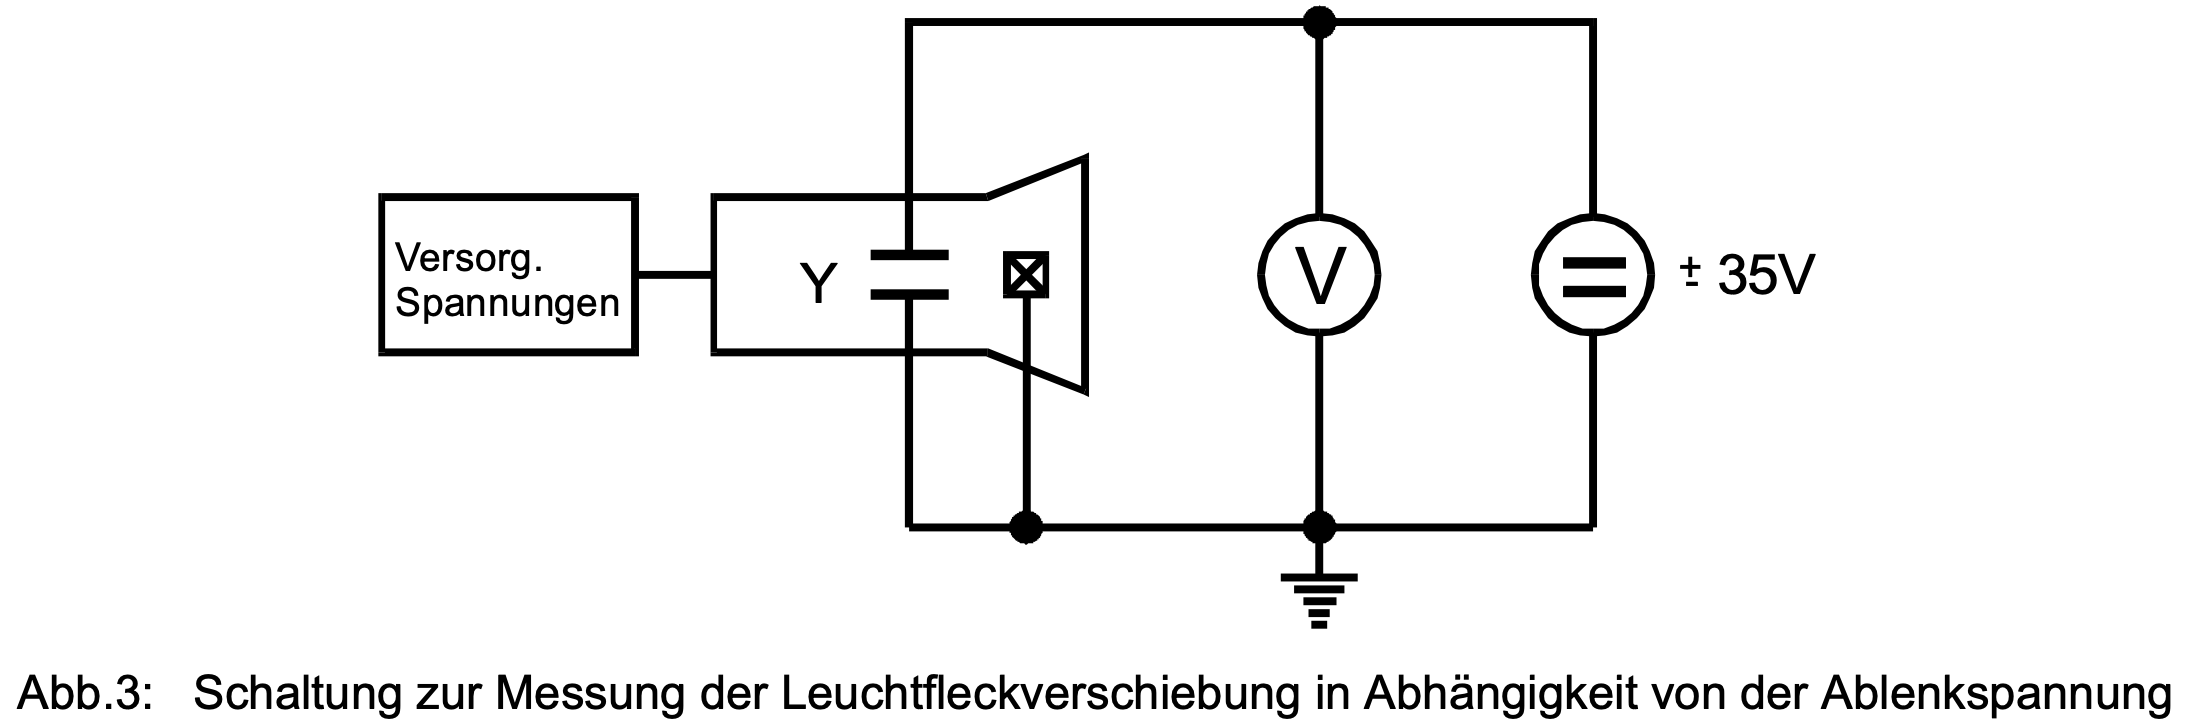
\includegraphics[width = 0.7\textwidth]{bilder/Schaltung.png}
    \caption{Eine Schaltung}
\end{figure}
Im zweiten Teil des Versuchs soll der Kathodenstrahl-Oszillograph getestet werden.
Um stehende Bilder der Sinusfrequenz zu erhalten wird dazu die Sägezahnspannung variiert bis die Synchronisationsbedingung erfüllt ist.
Es wird versucht durch passendes einstellen der Spannungen die Fälle für $n = \sfrac{1}{2},1,2$ und $3$ zu realisieren und die entsprechende Frequenz für $\nu_{Sä}$ abzulesen.
Außerdem soll jeweils die maximale Strahlauslenkung in Y-Richtung bei einer konstanten Beschleunigungsspannung ausgemessen werden.